\chapter{繰り返し処理をもう一歩：配列を操作する}
\label{chap:iteration-again}

この章では、第7章で学んだ\texttt{for}文や\texttt{while}文を土台にして、配列をより柔軟に扱う方法を学びます。これまでの章では、配列に入っている値を番号で取り出すことが多くありました。この章では、配列の中身を順番に読む\texttt{for...of}、配列の末尾や先頭に要素を追加・削除する\texttt{push}、\texttt{pop}、\texttt{shift}、\texttt{unshift}を中心に扱います。最後に、番号やプロパティ名を読む\texttt{for...in}も紹介します。

\section{この章の概要}

ゲームや作品を作っていると、最初から数が決まっていないものを扱いたくなります。たとえば、画面に出ている効果、取得したアイテム、最近押されたキー、ログメッセージなどは、実行中に増えたり減ったりします。TypeScriptの配列では、プログラムの実行中にも要素を追加したり削除したりできます。このような場面では、配列を番号で並んだ値の集まりとして見るだけでなく、必要に応じて中身が変わるリストとして扱えると便利です。

この章で扱う主な内容は次の通りです。

\begin{itemize}
    \item \texttt{for...of}で配列の値を順番に読む
    \item \texttt{push}と\texttt{pop}で末尾を操作する
    \item \texttt{shift}と\texttt{unshift}で先頭を操作する
    \item スタックとキューの考え方を知る
    \item p5.jsの作品で、増減するリストを使う
    \item \texttt{for...in}で番号やプロパティ名を読む
\end{itemize}

\begin{pointbox}{この章の位置づけ}
この章の内容は、配列を使ったゲームやシミュレーションを作るときに役立ちます。ただし、最初からすべてを暗記する必要はありません。\texttt{for...of}は「値を順番に読む」、\texttt{push}は「後ろに追加する」くらいの感覚から始めましょう。
\end{pointbox}

\section{\texttt{for...of}で値を順番に読む}

配列の中身をすべて使いたいとき、これまでは\texttt{for}文と添字を組み合わせていました。\texttt{for...of}を使うと、添字を自分で管理しなくても、配列の値を先頭から順番に取り出せます。

\begin{listing}[htbp]
\inputminted{ts}{listings/chapter18-iteration/for-of-colors.ts}
\caption{\texttt{for...of}で色のリストを順番に使う}
\label{lst:chapter18-iteration-for-of-colors}
\end{listing}

\texttt{for (const circleColor of circleColors)}は、「\texttt{circleColors}の中から、値を1つずつ\texttt{circleColor}として取り出す」と読みます。配列の何番目かを気にしなくてよいので、すべての値に同じ処理をしたいときに読みやすくなります。

\begin{figure}[htbp]
    \centering
    \begin{tikzpicture}[x=1.6cm,y=1cm]
        \foreach \i/\name/\col in {0/red/red!60,1/green/green!60,2/blue/blue!55,3/yellow/yellow!70} {
            \draw[fill=\col] (\i,0) rectangle +(1,0.7);
            \node at (\i+0.5,0.35) {\small \name};
        }
        \draw[->,thick] (0.5,-0.25) -- (0.5,-0.9);
        \draw[->,thick] (1.5,-0.25) -- (1.5,-0.9);
        \draw[->,thick] (2.5,-0.25) -- (2.5,-0.9);
        \draw[->,thick] (3.5,-0.25) -- (3.5,-0.9);
        \node[draw,rounded corners,fill=white] at (2,-1.25) {\texttt{circleColor}に1つずつ入る};
    \end{tikzpicture}
    \caption{\texttt{for...of}は配列の値を順番に取り出す}
    \label{fig:chapter18-iteration-for-of}
\end{figure}

\begin{notebox}{何番目かが必要なら普通の\texttt{for}文も使う}
\texttt{for...of}は値を取り出すには便利ですが、「何番目の値か」を使いたいときは、これまで通り\texttt{for (let index = 0; ...)}の形が分かりやすい場合があります。目的によって使い分けます。
\end{notebox}

\section{末尾に追加する\texttt{push}と末尾から取り出す\texttt{pop}}

\texttt{push}と\texttt{pop}は、配列そのものの中身を変えるメソッドです。\texttt{push}は配列の末尾に要素を追加し、追加したあとの配列の長さを返します。\texttt{pop}は配列の末尾から要素を1つ取り出し、その要素を返します。

\begin{figure}[htbp]
    \centering
    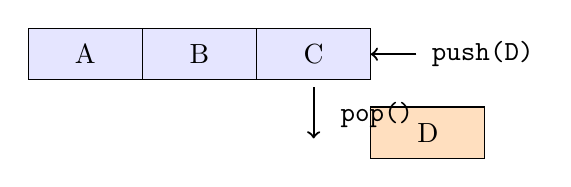
\begin{tikzpicture}[x=1.45cm,y=1cm]
        \foreach \i/\name in {0/A,1/B,2/C} {
            \draw[fill=blue!10] (\i,0) rectangle +(1,0.65);
            \node at (\i+0.5,0.32) {\name};
        }
        \draw[->,thick] (3.4,0.32) -- (3.0,0.32);
        \node[right] at (3.45,0.32) {\texttt{push(D)}};
        \draw[fill=orange!25] (3,-1.0) rectangle +(1,0.65);
        \node at (3.5,-0.68) {D};
        \draw[->,thick] (2.5,-0.1) -- (2.5,-0.75);
        \node[right] at (2.65,-0.45) {\texttt{pop()}};
    \end{tikzpicture}
    \caption{\texttt{push}と\texttt{pop}は配列の末尾を操作する}
    \label{fig:chapter18-iteration-push-pop}
\end{figure}

\begin{listing}[htbp]
\inputminted{ts}{listings/chapter18-iteration/push-pop-stack.ts}
\caption{\texttt{push}と\texttt{pop}で操作履歴を扱う}
\label{lst:chapter18-iteration-push-pop-stack}
\end{listing}

\texttt{push}は追加後の長さを返しますが、このサンプルでは戻り値を使わず、追加したという操作だけに注目しています。\texttt{pop}の戻り値は、取り出した要素です。ただし、配列が空のときに\texttt{pop}すると、値が取り出せないため\texttt{undefined}になります。この章では、初学者が安全に読めるように、\texttt{commands.length > 0}で空ではないことを確認してから\texttt{pop}しています。

\begin{pointbox}{スタックという考え方}
最後に入れたものを最初に取り出す構造を、スタックと呼びます。ゲームでは、直前の操作を取り消す、画面の状態を戻す、履歴をたどる、といった場面で似た考え方を使います。
\end{pointbox}

\section{先頭を操作する\texttt{shift}と\texttt{unshift}}

\texttt{shift}と\texttt{unshift}も、配列そのものの中身を変えるメソッドです。\texttt{shift}は配列の先頭から要素を1つ取り出し、その要素を返します。\texttt{unshift}は配列の先頭に要素を追加し、追加したあとの配列の長さを返します。末尾ではなく先頭を動かすため、時間の順番を持つリストや待ち行列を表すときに使えます。

\begin{figure}[htbp]
    \centering
    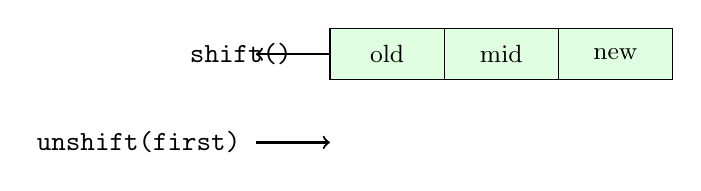
\begin{tikzpicture}[x=1.45cm,y=1cm]
        \node[left] at (-0.25,0.32) {\texttt{shift()}};
        \draw[->,thick] (0.0,0.32) -- (-0.65,0.32);
        \foreach \i/\name in {0/old,1/mid,2/new} {
            \draw[fill=green!12] (\i,0) rectangle +(1,0.65);
            \node at (\i+0.5,0.32) {\small \name};
        }
        \draw[->,thick] (-0.65,-0.8) -- (0,-0.8);
        \node[left] at (-0.7,-0.8) {\texttt{unshift(first)}};
    \end{tikzpicture}
    \caption{\texttt{shift}と\texttt{unshift}は配列の先頭を操作する}
    \label{fig:chapter18-iteration-shift-unshift}
\end{figure}

\begin{listing}[htbp]
\inputminted{ts}{listings/chapter18-iteration/shift-unshift-queue.ts}
\caption{\texttt{shift}と\texttt{push}でメッセージを古い順に処理する}
\label{lst:chapter18-iteration-shift-unshift-queue}
\end{listing}

このサンプルでは、\texttt{messages.push(...)}で新しいメッセージを末尾に追加し、\texttt{messages.shift()}で古いメッセージから取り出しています。\texttt{shift}したときに配列が空なら、戻り値は\texttt{undefined}になります。先に入ったものから順番に処理する構造を、キューと呼びます。

\begin{notebox}{\texttt{shift}と\texttt{unshift}は先頭を動かす}
\texttt{push}と\texttt{pop}は末尾、\texttt{shift}と\texttt{unshift}は先頭を操作します。名前だけでは向きが分かりにくいため、最初は図\ref{fig:chapter18-iteration-push-pop}と図\ref{fig:chapter18-iteration-shift-unshift}を見ながら確認しましょう。
\end{notebox}

\section{p5.jsで増減するリストを使う}

最後に、p5.jsの作品らしいサンプルとして、クリックした場所に小さな光を追加し、古い光から消していくプログラムを作ります。クリックするたびに配列へ追加し、数が多くなったら先頭から削除します。

\begin{listing}[htbp]
\inputminted[firstline=1,lastline=35]{ts}{listings/chapter18-iteration/click-sparkles.ts}
\caption{クリックで追加される光のクラス}
\label{lst:chapter18-iteration-sparkle-class}
\end{listing}

\begin{listing}[htbp]
\inputminted[firstline=37,lastline=73]{ts}{listings/chapter18-iteration/click-sparkles.ts}
\caption{\texttt{push}と\texttt{shift}で光のリストを管理する}
\label{lst:chapter18-iteration-sparkle-sketch}
\end{listing}

\texttt{sparkles.push(new Sparkle(...))}は、新しい光を末尾に追加します。\texttt{sparkles.length > maxSparkleCount}になったら、\texttt{sparkles.shift()}で古い光を先頭から削除します。こうすると、画面上に残る光の数を一定以下にできます。

\texttt{for...of}は、画面にあるすべての光を更新・描画するために使っています。光の番号は必要なく、光そのものを順番に使いたいので、\texttt{for...of}が読みやすい場面です。

\section{\texttt{for...in}で番号や名前を読む}

\texttt{for...in}は、配列やオブジェクトの「キー」を順番に取り出します。ここまでに扱った\texttt{for...of}は値を順番に取り出す構文でした。それに対して、\texttt{for...in}は値そのものではなく、値を取り出すための番号や名前を取り出します。少し考え方が違うため、この章では最後に紹介します。

\begin{listing}[htbp]
\inputminted{ts}{listings/chapter18-iteration/for-in-array.ts}
\caption{\texttt{for...in}で配列の番号を取り出す}
\label{lst:chapter18-iteration-for-in-array}
\end{listing}

\texttt{for...in}で取り出した\texttt{indexText}は文字列です。数値として使いたいときは、\texttt{Number(indexText)}で数値に変換します。この変換が必要になるため、配列の中身を読むだけなら\texttt{for...of}の方が書きやすいことが多いです。

\begin{listing}[htbp]
\inputminted{ts}{listings/chapter18-iteration/for-in-object.ts}
\caption{\texttt{for...in}で得点表の名前を取り出す}
\label{lst:chapter18-iteration-for-in-object}
\end{listing}

このサンプルでは、プレイヤー名をキー、得点を値として持つオブジェクトを使っています。\texttt{for...in}は、\texttt{"Aoi"}、\texttt{"Ren"}、\texttt{"Mika"}のようなキーを順番に取り出します。そのキーを使って\texttt{scores[playerName]}と書くと、対応する得点を取り出せます。

\begin{pointbox}{配列なら\texttt{for...of}、キーが欲しいなら\texttt{for...in}}
配列の値を順番に使いたいときは、まず\texttt{for...of}を考えます。配列の番号や、オブジェクトのプロパティ名が必要なときは、\texttt{for...in}を使う候補になります。
\end{pointbox}

\section{よくある間違い}

配列を増減させる処理では、何をどちら側から入れ、何をどちら側から取り出すのかが分からなくなりやすいです。名前と図を結びつけて、落ち着いて確認しましょう。

\begin{mistakebox}{\texttt{for...in}で値が取り出せると思ってしまう}
\texttt{for...in}で配列を読むと、取り出されるのは値そのものではなく番号です。値を読みたい場合は、基本的には\texttt{for...of}を使います。
\end{mistakebox}

\begin{mistakebox}{空の配列から\texttt{pop}や\texttt{shift}をしてしまう}
空の配列から値を取り出そうとすると、期待した値は得られません。取り出す前に\texttt{array.length > 0}を確認すると安全です。
\end{mistakebox}

\begin{mistakebox}{追加と削除の向きを混同する}
\texttt{push}と\texttt{pop}は末尾を操作します。\texttt{shift}と\texttt{unshift}は先頭を操作します。スタックなら\texttt{push}と\texttt{pop}、キューなら\texttt{push}と\texttt{shift}の組み合わせがよく使われます。
\end{mistakebox}

\begin{mistakebox}{\texttt{draw}の中で毎フレーム追加してしまう}
\texttt{draw}は何度も実行されます。\texttt{draw}の中で毎回\texttt{push}すると、配列がどんどん大きくなります。クリックやキー入力など、必要なタイミングだけで追加するようにします。
\end{mistakebox}

\section{まとめ}

この章では、配列を順番に読む\texttt{for...of}、キーを読む\texttt{for...in}、配列の末尾や先頭を操作する\texttt{push}、\texttt{pop}、\texttt{shift}、\texttt{unshift}を学びました。これらを使うと、数が変化するアイテム、効果、ログ、操作履歴などを扱いやすくなります。

次の章では、Life Gameを題材にして、同じ結果を得るための処理の進め方を工夫します。この章で学んだ「リストに記録する」考え方は、変化した場所を保存する処理にもつながります。

\section{演習問題}

この章の演習では、配列を読むだけでなく、実行中に増やしたり減らしたりする練習をします。どの操作が先頭を使い、どの操作が末尾を使うのかを意識しながら進めてください。

\begin{enumerate}
    \item \texttt{for...of}を使って、文字列の配列に入った名前をすべて表示してください。
    \item 数値の配列を作り、\texttt{for...of}を使って合計を求めてください。
    \item 文字列の配列に\texttt{push}で新しい値を追加し、追加前後の\texttt{length}を表示してください。
    \item \texttt{pop}を使って、最後に追加した値を取り出してください。
    \item \texttt{push}と\texttt{shift}を使って、古いメッセージから順に取り出すプログラムを作ってください。
    \item \texttt{unshift}を使って、重要なメッセージをリストの先頭に追加してください。
    \item クリックした位置を配列に保存し、\texttt{for...of}で全部の点を描くプログラムを作ってください。
    \item 点の数が20個を超えたら、\texttt{shift}で古い点を消すようにしてください。
    \item \texttt{for...in}を使って、配列の番号と値を両方表示してください。
    \item 挑戦問題として、最近押したキーを5個だけ表示するプログラムを作ってください。新しいキーを\texttt{push}し、6個以上になったら\texttt{shift}で古いキーを消します。
\end{enumerate}
